%! TeX program = lualatex
\documentclass[main]{subfiles}

\begin{document}

\title[AutoML: HPO]{Evolutionary Algorithms}
\subtitle{Mutate and Crossover Your Way to Better Performance}
\author[Lars Kotthoff]{Lars Kotthoff}
\date{}

%\institute{}
%\date{}
	
	\maketitle
	

\begin{frame}{Evolutionary Algorithms}
    \begin{itemize}
        \item Inspired by evolution in nature
        \item Create an initial population of configurations
        \item Repeat:
            \begin{itemize}
                \item Evaluate the ``fitness'' of the configurations in the
                    population by measuring their performances
                \item Crossover: combine two configurations, e.g.\ by taking
                    some hyperparameter values from one and the rest from the
                    other
                \item Mutation: randomly change the hyperparameter values of a
                    configuration
                \item Promote configurations to the next ``generation,'' i.e.\
                    choose which ones will ``survive''
            \end{itemize}
    \end{itemize}
\end{frame}

%----------------------------------------------------------------------

\begin{frame}{Evolutionary Algorithms Example}
    \begin{itemize}
        \item Randomly sample the initial population
        \item From the top-performing half of configurations
            \begin{itemize}
                \item Crossover configurations by taking the first half of all
                    hyperparameter values from the first, the second from
                    the second
                \item Mutate a small number of configurations by adding
                    Gaussian random noise, centered on the current value, to
                    a randomly-chosen hyperparameter
            \end{itemize}
        \item Crossover and mutate until the same number of configurations
            as in the previous population have been generated
        \item Repeat until no improvement observed
    \end{itemize}
\end{frame}


\begin{frame}{Evolutionary Algorithms Example}
    XGBoost hyperparameter tuning on OpenML dataset 11 (balance-scale)
    \begin{center}
        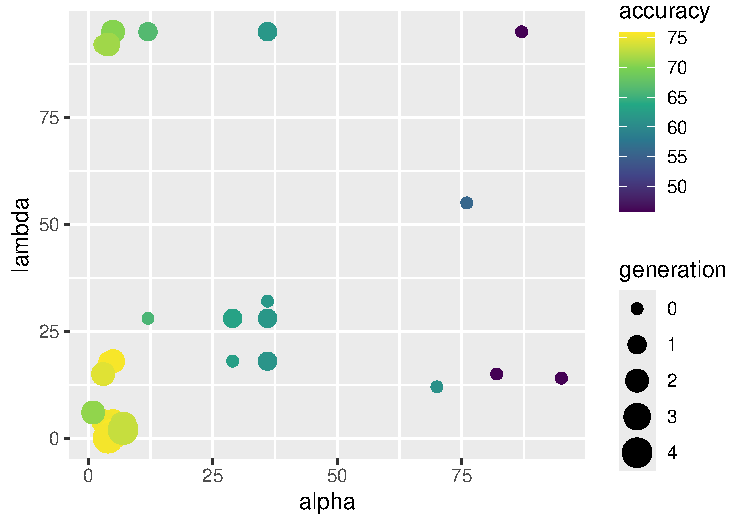
\includegraphics[height=.9\textheight]{images/ga}
    \end{center}
\end{frame}

%----------------------------------------------------------------------

\begin{frame}{Evolutionary Algorithms Considerations}
    \begin{itemize}
        \item Advantages
            \begin{itemize}
                \item Conceptually simple
                \item Can work with many different representations (e.g.\ full
                    ML pipelines and their components)
                \item Adaptive
                \item Easily parallelizable
            \end{itemize}
        \item Disadvantages
            \begin{itemize}
                \item Need to define population size, number of generations, how
                    crossover and mutation should be done, the relative
                    frequency of crossover and mutation, what configurations
                    should be used to generate survivors\ldots
                \item Can be quite slow to find well-performing configurations
            \end{itemize}
    \end{itemize}
\end{frame}

%----------------------------------------------------------------------

\begin{frame}{Summary} 
\begin{enumerate}
    \item Evolutionary Algorithms improve configurations by combining known good
        performers and random changes
    \item Can be applied to all types of configuration spaces
    \item Often quite resource-intensive
\end{enumerate}
\end{frame}

\end{document}
